\documentclass[10pt]{beamer}

\ifx\pdfoutput\undefined
% we are running LaTeX, not pdflatex
\usepackage{graphicx}
\else
% we are running pdflatex, so convert .eps files to .pdf
\usepackage{graphicx}
\usepackage{epstopdf}
\fi

\input{beihangbeamerstyle/beihangcolor}
\input{beihangbeamerstyle/beihangbeamerstyle}

\title{Neural image compression with scene graphs}
\author{道尔格\\
Beihang University (\texttt{ls1906205@buaa.edu.cn})}
\date{Thesis proposal defence, Beihang University, Fri  21 May 2021}


\begin{document}
%----------------------------------------------------------------------
% Title frame
\begin{frame}[plain]
    \maketitle
\end{frame}

%----------------------------------------------------------------------
% Outline frame
% PLEASE RUN pdflatex TWICE 
\begin{frame}
    \frametitle{Outline}
    \tableofcontents
\end{frame}
%%=====================================================================
% Section I
\section{Introduction}
%----------------------------------------------------------------------
% Content frame
\begin{frame}
    \frametitle{Introduction}

    \framesubtitle{Why I made this beamer style}
    \begin{block}{Image compression}
        Image compression is an important task in computer science and engineering.
        Two main approaches:
        \begin{itemize}
            \item Lossy (estimating information). JPEG etc.
            \item Lossless (compressing information). DEFLATE etc.
        \end{itemize}
        Discrete cosine transform (DCT), Huffman coding.
    \end{block}
\end{frame}
%----------------------------------------------------------------------
\begin{frame}
    \frametitle{Compression}
    \begin{columns}
        \begin{column}{0.5\textwidth}
            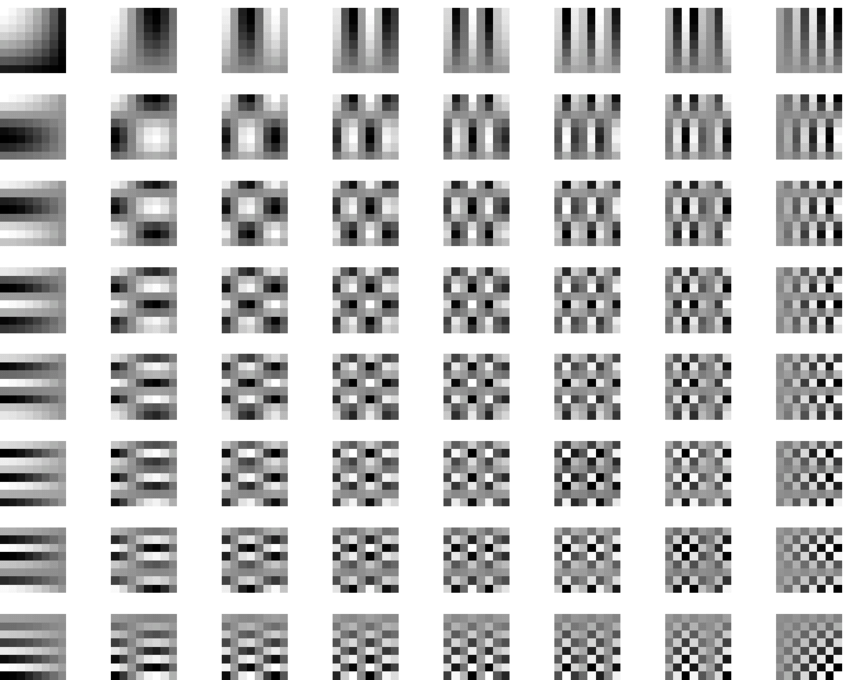
\includegraphics[width=\textwidth]{figure/2d-dct.png}
        \end{column}
        \begin{column}{0.5\textwidth}
            \begin{block}{Image compression}

                It is common to use DCT based methods in image compression. A popular implementation of Fourier transform for discrete functions is Discrete Cosine Transform.

                However this is not the only one approach. Instead of using a predefined polynomial to encode an image, it is possible to use neural networks to pack and unpack information.

            \end{block}
        \end{column}
    \end{columns}
\end{frame}

\begin{frame}
    \frametitle{Neural compression}
    There were several approaches to apply neural networks architecture in image compression. Take an autoencoder architecture as an example:
    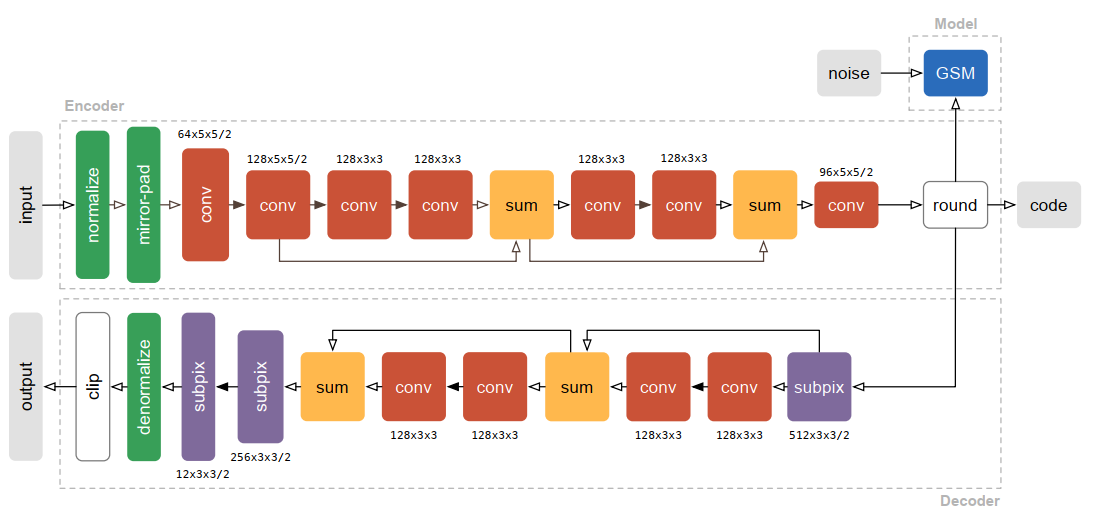
\includegraphics[width=\textwidth]{figure/neural-compression.png}
\end{frame}


\begin{frame}
    \frametitle{Image and sene gaph}
    \begin{columns}
        \begin{column}{0.5\textwidth}
            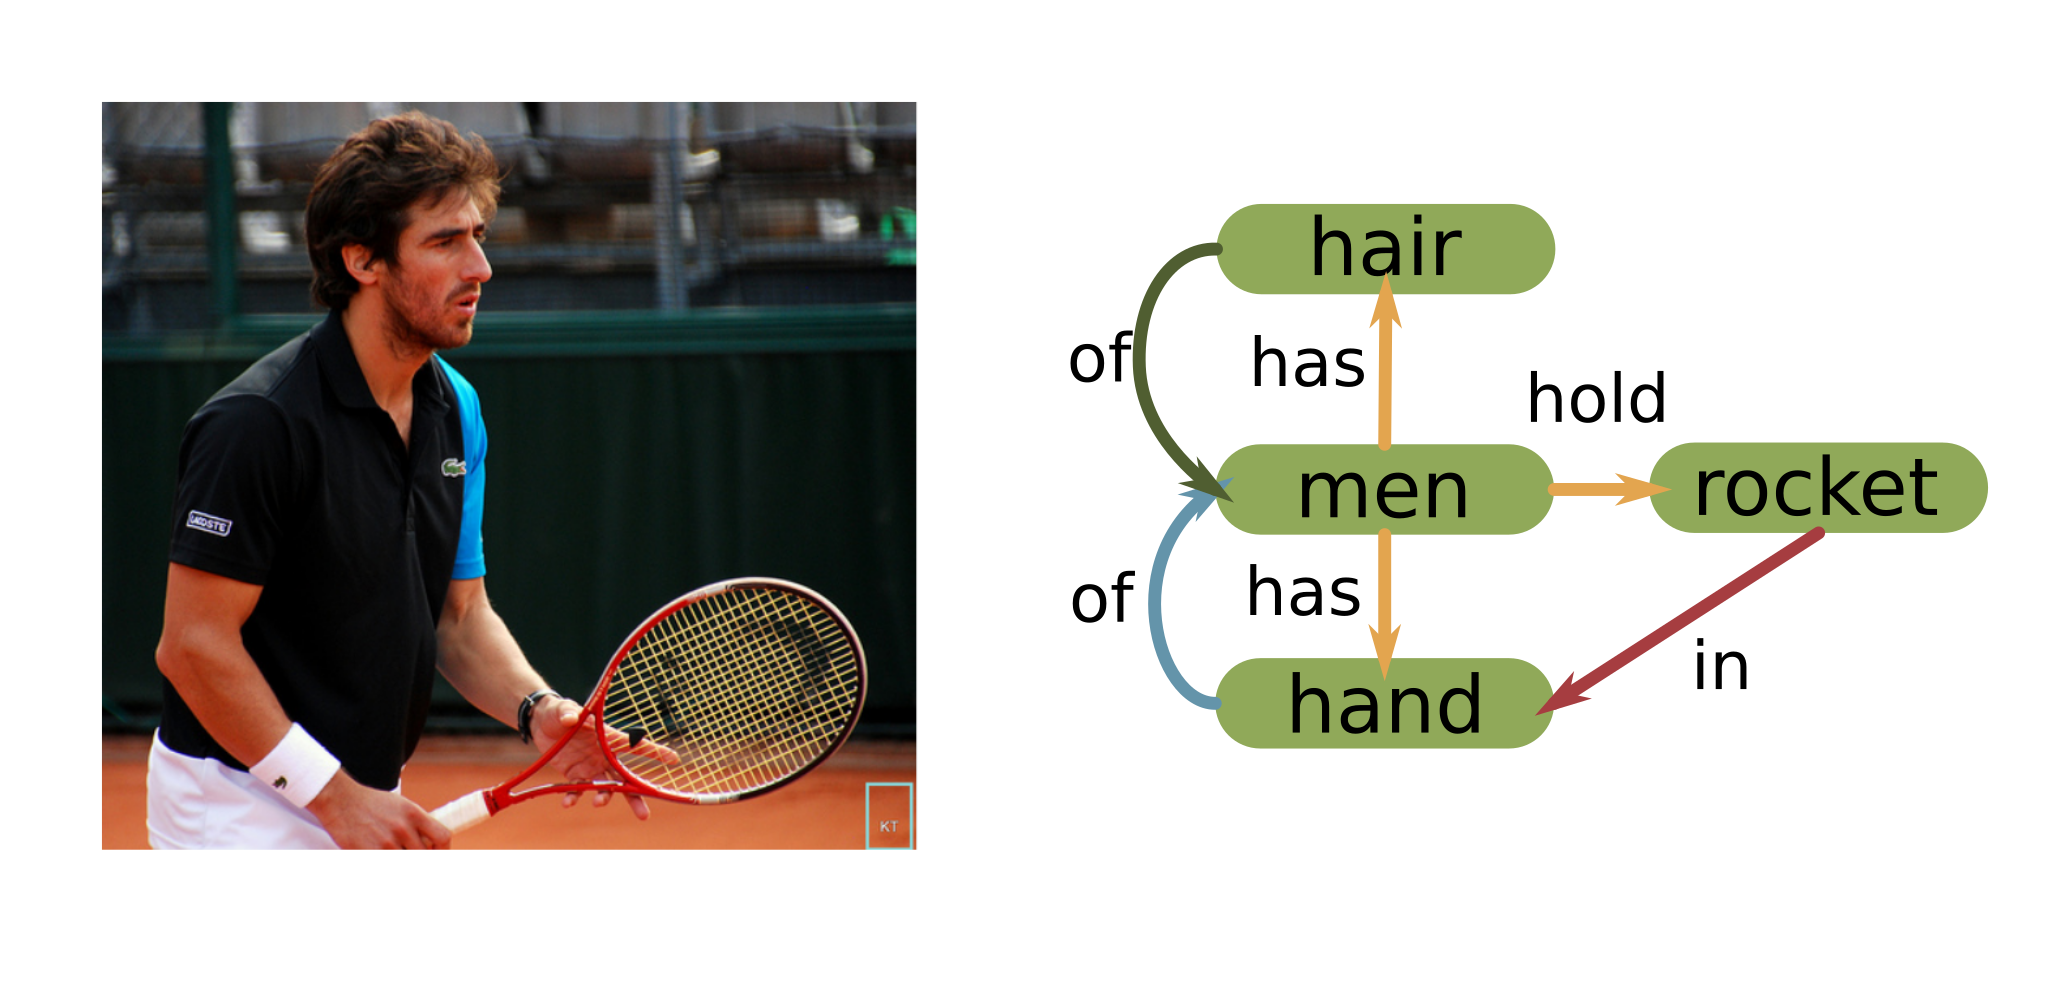
\includegraphics[width=\textwidth]{figure/image-and-scene-graph.png}
        \end{column}
        \begin{column}{0.5\textwidth}
            How do we memorize image or visual scene in our life. We do not operate in terms of pixels or object coordinates. More likely we use something like scheme, which describes the most important parts of an image.
            There are already algorithms capable to extract Scene Graphs form image. There are some approaches to generate an image from scene graphs. We can combine those two.
        \end{column}
    \end{columns}
\end{frame}

\end{document}


